
% v2-acmsmall-sample.tex, dated March 6 2012
% This is a sample file for ACM small trim journals
%
% Compilation using 'acmsmall.cls' - version 1.3 (March 2012), Aptara Inc.
% (c) 2010 Association for Computing Machinery (ACM)
%
% Questions/Suggestions/Feedback should be addressed to => "acmtexsupport@aptaracorp.com".
% Users can also go through the FAQs available on the journal's submission webpage.
%
% Steps to compile: latex, bibtex, latex latex
%
% For tracking purposes => this is v1.3 - March 2012
\documentclass[prodmode,acmtecs]{acmsmall} % Aptara syntax
\usepackage[spanish,polish]{babel}
\usepackage[T1]{fontenc}
\usepackage{fancyvrb}
\usepackage{graphicx,hyperref}
\newcommand\cutout[1]{}


\usepackage[table]{xcolor}
\usepackage[utf8]{inputenc}
\usepackage[parfill]{parskip}
\usepackage{tabulary}
\PassOptionsToPackage{hyphens}{url}
\usepackage{hyperref}    
\usepackage[capitalize]{cleveref}


% Metadata Information
% !!! TODO: SET THESE VALUES !!!
\acmVolume{0}
\acmNumber{0}
\acmArticle{CFP}
\acmYear{0}
\acmMonth{0}

\newcounter{colstart}
\setcounter{page}{4}

\RecustomVerbatimCommand{\VerbatimInput}{VerbatimInput}%
{
%fontsize=\footnotesize,
fontfamily=\rmdefault
}


\newcommand{\UnderscoreCommands}{%\do\verbatiminput%
\do\citeNP \do\citeA \do\citeANP \do\citeN \do\shortcite%
\do\shortciteNP \do\shortciteA \do\shortciteANP \do\shortciteN%
\do\citeyear \do\citeyearNP%
}

\usepackage[strings]{underscore}



% Document starts
\begin{document}


\setcounter{colstart}{\thepage}

\acmArticle{CFP}
\title{{\huge\sc SIGLOG Monthly 241}

 September 2023}
\author{DAVID PURSER\affil{University of Liverpool, UK}
\vspace*{-2.6cm}\begin{flushright}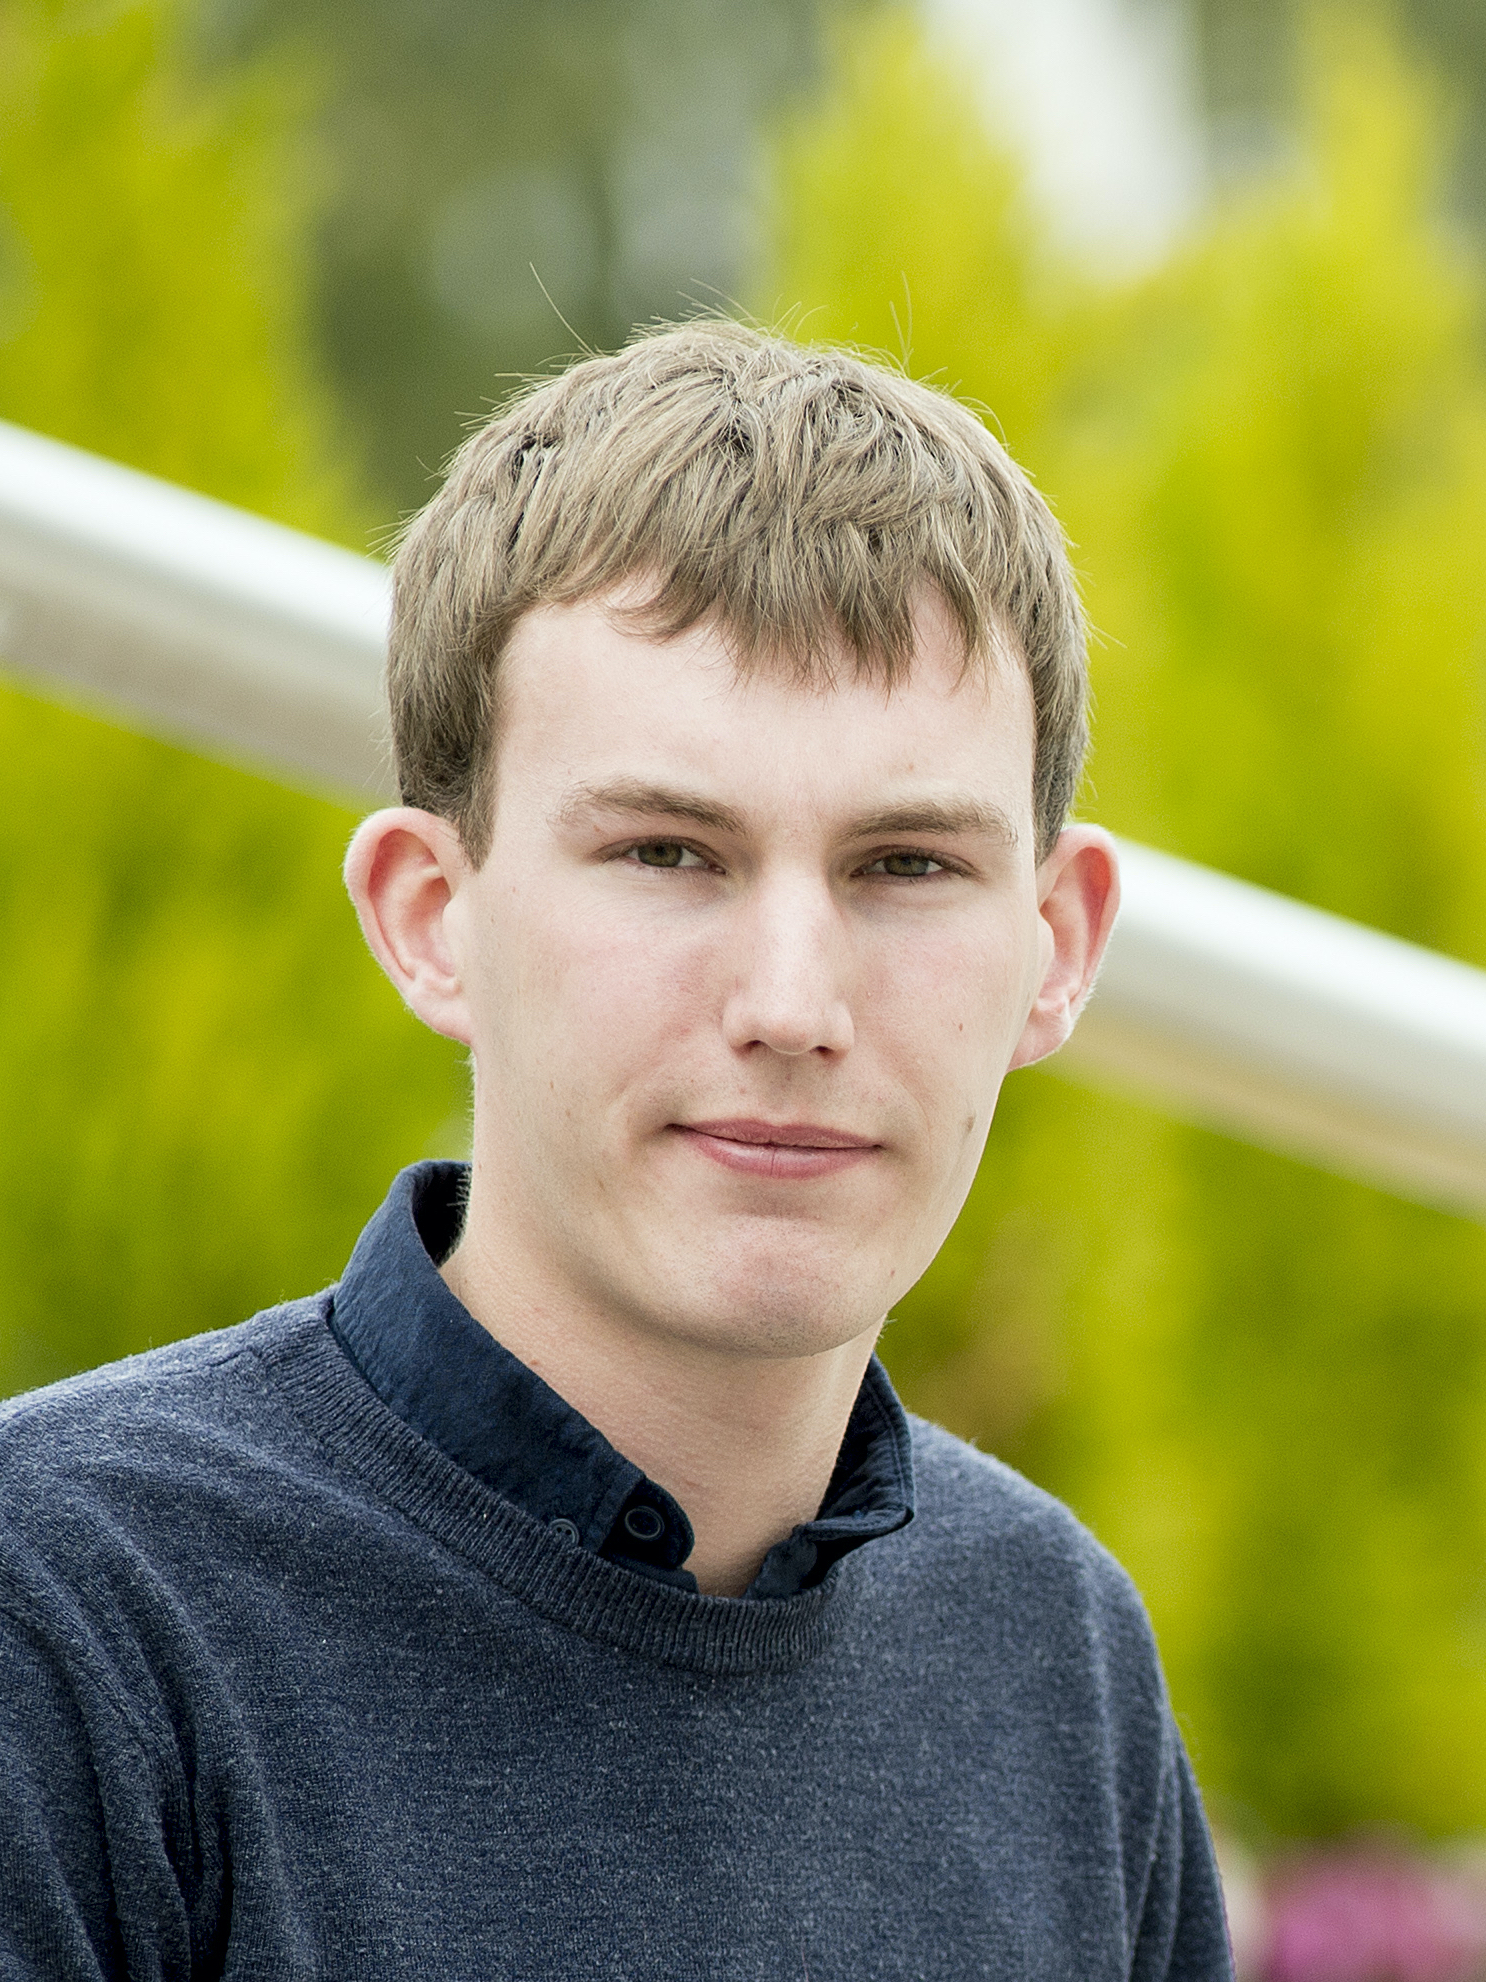
\includegraphics[width=30mm]{dp}\end{flushright}
}

\begin{abstract}
September 2023 edition of SIGLOG Monthly, featuring deadlines, calls and community announcements.
\end{abstract}


\maketitlee

\href{https://lics.siglog.org/newsletters/}{Past Issues}
 - 
\href{https://lics.siglog.org/newsletters/inst.html}{How to submit an announcement}
\section{Table of Content}\begin{itemize}\item DEADLINES (\cref{deadlines}) 
 
\item SIGLOG MATTERS 
 
\begin{itemize}\item Research Highlights (\cref{ResearchHighlights})
\end{itemize} 
\item CALLS 
 
\begin{itemize}\item BEWARE-23 (CALL FOR PAPERS) (\cref{BEWARE23})
\item GandALF 23 (CALL FOR PARTICIPATION) (\cref{GandALF23})
\item TIME 2023 (CALL FOR PARTICIPATION) (\cref{TIME2023})
\item FSCD 2024 (CALL FOR PAPERS) (\cref{FSCD2024})
\end{itemize} 
\end{itemize}\section{Deadlines}\label{deadlines}\rowcolors{1}{white}{gray!25}\begin{tabulary}{\linewidth}{LL}VMCAI 2024:  & Sep 07, 2023 (Paper, extended) \\
BEWARE-23:  & Sep 10, 2023 (Paper) \\
CPP 2024:  & Sep 12, 2023 (Abstract), Sep 19, 2023 (Paper) \\
ICDT 2024:  & Sep 13, 2023 (Cycle 2 Abstract), Sep 20, 2023 (Cycle 2 Full) \\
OVERLAY 2023:  & Sep 22, 2023 (Paper, extended) \\
FLOPS 2024:  & Dec 06, 2023 (Abstract due), Dec 13, 2023 (Papers due) \\
DEON2023:  & Jan 07, 2024 (Paper) \\
FSCD 2024:  & Feb 05, 2024 (Abstract), Feb 12, 2024 (Paper) \\
\end{tabulary}
\section{Research Highlights}\label{ResearchHighlights}CALL FOR NOMINATIONS 

\begin{itemize}\item  The Research Highlights section of the Communications of the ACM aims to provide readers with a collection of outstanding research articles, selected from the broad spectrum of computing-research conferences.  
 
  Starting this year, SIGLOG is an approved nominating organization for the Research Highlights section. Accordingly, the Research Highlights Committee of ACM SIGLOG is looking for nominations of high-quality papers from the past year in the areas related to SIGLOG that can be appreciated by the broader public of the computer science research community.  
 
  There are three key criteria for a good Research Highlights paper: 
 
\begin{itemize}\item  The work must be a strong, novel research contribution.
\item  It should be of broad interest to the computing community. (This means the selection criterion is not necessarily the same as that for Best Papers and other awards, which can recognize papers that are quite narrow and focused on a very small community.)
\item  Papers should have that little extra “pop” that sets them apart even from other strong results in their field. A nomination should suggest that you think a paper should be one of the most widely read papers in computer science.
\end{itemize} 
  It should be noted that a Research Highlights paper is not the “journal version” of a conference paper. Instead, it is essentially a reprint of the paper and does not preclude a later journal version. 
 
   There is no deadline for submitting nominations, but since it is the first year SIGLOG is participating in the Research Highlights, we would like to review initial nominations as early as possible.  
 
   Nominations can be made using this form: \href{https://docs.google.com/forms/d/e/1FAIpQLSf_EzPU1yK8k3quGyHhiUpTt_OLqEiylgwJ12UaxUFuKqnMcw/viewform}{https://docs.google.com/forms/d/e/1FAIpQLSf\_EzPU1yK8k3quGyHhiUpTt\_OLqEiylgwJ12UaxUFuKqnMcw/viewform} 
 
   We appreciate your cooperation and hope to see many SIGLOG papers published at the Research Highlights section of the Communications of the ACM! 
 
\end{itemize}\section{BEWARE-23: The 2nd international workshop on the emerging ethical aspects of AI, with a focus on Bias, Risk, Explainability and the role of Logic and Computational Logic}\label{BEWARE23}  \href{https://sites.google.com/view/beware2023}{https://sites.google.com/view/beware2023} \\ 
  BEWARE23 is co-located with the AIxIA 2023 conference.\\ 
CALL FOR PAPERS 

\begin{itemize}\item  Aims and Scope 
 
  Current AI applications do not guarantee objectivity and are riddled with biases and legal difficulties. AI systems need to perform safely, but problems of opacity, bias and risk are pressing. Definitional and foundational issues about what kinds of bias and risks are involved in opaque AI technologies are still very much open. Moreover, AI is challenging Ethics and brings the need to rethink the basis of Ethics. In this context, it is natural to look for theories, tools and technologies to address the problem of automatically detecting biases and implementing ethical decision-making. Logic, Computational Logic and formal ontologies have great potential in this area of research, as logic rules are easily comprehensible by humans and favour the representation of causality, which is a crucial aspect of ethical decision-making. Nonetheless, their expressivity and transparency need to be integrated within conceptual taxonomies and socio-economic analyses that place AI technologies in their broader context of application and determine their overall impact. This workshop addresses issues of logical, ethical and epistemological nature in AI through the use of interdisciplinary approaches. We aim to bring together researchers in AI, philosophy, ethics, epistemology, social science, etc., to promote collaborations and enhance discussions towards the development of trustworthy AI methods and solutions that users and stakeholders consider technologically reliable and socially acceptable. 
 
   The workshop invites submissions from computer scientists, philosophers, economists and sociologists wanting to discuss contributions ranging from the formulation of epistemic and normative principles for AI, their conceptual representation in formal models, to their development in formal design procedures and translation into computational implementations. 
 
\item  Topics of interest include, but are not at all limited to: 
 
\begin{itemize}\item  Conceptual and formal definitions of bias, risk and opacity in AI
\item  Epistemological and normative principles for fair and trustworthy AI
\item  Ethical AI and the challenges brought by AI to Ethics
\item  Explainable AI
\item  Uncertainty in AI
\item  Ontological modelling of trustworthy as opposed to biased AI systems
\item  Defining trust and its determinants for implementation in AI systems
\item  Methods for evaluating and comparing the performances of AI systems
\item  Approaches to verification of ethical behaviour
\item  Logic Programming Applications in Machine Ethics
\item  Integrating Logic Programing with methods for Machine Ethics and Explainable AI
\end{itemize} 
\item  Submission 
 
  See full call: \href{https://sites.google.com/view/beware2023/call-for-papers?authuser=0}{https://sites.google.com/view/beware2023/call-for-papers?authuser=0} 
 
\item  Important Dates 
 
\rowcolors{1}{white}{gray!25}\begin{tabulary}{\linewidth}{LL}Paper submission:  & Sep 10, 2023 \\
Notification:  & Oct 06, 2023 \\
Camera ready:  & Oct 20, 2023 \\
\end{tabulary}
 
\end{itemize}\section{GandALF 23: Fourteenth International Symposium on Games, Automata, Logics, and Formal Verification}\label{GandALF23}  Udine, Italy, Sept 18-20, 2023\\ 
  \href{https://gandalf23.uniud.it/}{https://gandalf23.uniud.it/}\\ 
CALL FOR PARTICIPATION 

\begin{itemize}\item  Registration is finally open for the Fourteenth International Symposium on Games, Automata, Logics, and Formal Verification (GandALF 23), to be held in Udine (Italy) on September 18-20, 2023. 
 
\item  We invite you to attend GandALF 2023. We will offer a very exciting technical and social program, which includes 15 contributed talks, 4 invited talks by renowned international theoretical computer scientists: 
 
\begin{itemize}\item  Weighted Automata At The Border Of Decidability by Laure Daviaud – University of East Anglia (UK),
\item  Complexity Aspects Of Logics In Team Semantics by Juha Kontinen – University of Helsinki (Finland),
\item  Strategic Reasoning Under Imperfect Information – The Case Of Synchronous Recall by Sophie Pinchinat IRISA/University of Rennes (France),
\item  The Church Synthesis Problem Over Continuous Time by Alexander Rabinovich – Tel Aviv University (Israel),
\end{itemize} 
  and an enchanting boat trip and dinner at a traditional Casone (check it out at \href{https://gandalf23.uniud.it/excursion/}{https://gandalf23.uniud.it/excursion/}). 
 
\item  To register to the conference, follow the instructions at \href{https://gandalf23.uniud.it/registration/}{https://gandalf23.uniud.it/registration/}. 
 
   For more details about GandALF 2023 and about how to organize your visit to Udine, check our webpage (\href{https://gandalf23.uniud.it/}{https://gandalf23.uniud.it/}). The full program will be published soon. 
 
\end{itemize}\section{TIME 2023: 30th International Symposium on Temporal Representation and Reasoning}\label{TIME2023}  September 25-26, 2023 at NCSR 'Demokritos' in Athens, Greece\\ 
  \href{https://cer.iit.demokritos.gr/events/time23/}{https://cer.iit.demokritos.gr/events/time23/}\\ 
CALL FOR PARTICIPATION 

\begin{itemize}\item  The TIME International Symposium brings together researchers from different disciplines of Computer Science working on temporal aspects of computational systems. 
 
\begin{itemize}\item  We are glad to announce that TIME will be back to an in-person conference! We look forward to welcoming the TIME community to Athens after 3 years of online events.
\item  TIME 2023 features 12 regular papers, 9 extended abstracts, and 2 invited talks.
\end{itemize} 
\item  Registration is now open 
 
\begin{itemize}\item  TIME 2023 has both physical registration as well as a remote-participation option
\item  The registration fee for physical participation is 300 Euros, the registration fee for remote participation is 50 Euros.
\item  Register at: \href{https://cer.iit.demokritos.gr/events/time23/#registration}{https://cer.iit.demokritos.gr/events/time23/\#registration}
\end{itemize} 
\item  Invited Speakers 
 
\begin{itemize}\item  Thomas Eiter, TU Vienna, Austria: Asynchronous Temporal Equilibrium Logic
\item  Laura Nenzi, University of Trieste, Italy: Learning Temporal Logic Formulas from Time-series Data
\end{itemize} 
\item  Program 
 
\begin{itemize}\item  Please find the program at: \href{https://cer.iit.demokritos.gr/events/time23/#program}{https://cer.iit.demokritos.gr/events/time23/\#program}
\end{itemize} 
\end{itemize}\section{FSCD 2024: Ninth International Conference on Formal Structures for Computation and Deduction}\label{FSCD2024}  July 10-13, 2024, Tallinn, Estonia\\ 
  \href{https://fscd-conference.org/2024}{https://fscd-conference.org/2024}\\ 
CALL FOR PAPERS 

\begin{itemize}\item  IMPORTANT DATES (AoE)  
 
\rowcolors{1}{white}{gray!25}\begin{tabulary}{\linewidth}{LL}Abstract:  & Feb 05, 2024 \\
Paper submission:  & Feb 12, 2024 \\
Rebuttal:  & Apr 2-6, 2024 \\
Notification:  & Apr 22, 2024 \\
Final version:  & May 06, 2024 \\
\end{tabulary}
 
\item  OVERVIEW 
 
  FSCD (\href{https://fscd-conference.org/}{https://fscd-conference.org/}) covers all aspects of formal structures for computation and deduction from theoretical foundations to applications. Building on two communities, RTA (Rewriting Techniques and Applications) and TLCA (Typed Lambda Calculi and Applications), FSCD embraces their core topics and broadens their scope to closely related areas in logic, models of computation, semantics and verification in new challenging areas. 
 
\item  TOPICS 
 
  The suggested, but not exclusive, list of topics for submission is: 
 
\begin{itemize}\item  Calculi: Rewriting systems (string, term, higher-order, graph, conditional, modulo, infinitary, etc.); Lambda calculus; Logics (first-order, higher-order, equational, modal, linear, classical, constructive, etc.); Proof theory (natural deduction, sequent calculus, proof nets, etc.); Type theory and logical frameworks; Homotopy type theory; Process algebras (synchronous, asynchronous, static and dynamic semantics with and without time, etc.); Quantum calculi.
\item  Methods in Computation and Deduction: Type systems (polymorphism, dependent, recursive, intersection, session, etc.); Induction, coinduction; Matching, unification, completion, orderings; Strategies (normalization, completeness, etc.); Tree automata; Model building and model checking; Proof search and theorem proving; Constraint solving and decision procedures.
\item  Semantics: Operational semantics and abstract machines; Game Semantics and applications; Domain theory and categorical models; Quantitative models (timing, probabilities, etc.); Quantum computation and emerging models in computation.
\item  Algorithmic Analysis and Transformations of Formal Systems: Type inference and type checking; Abstract Interpretation; Complexity analysis and implicit computational complexity; Checking termination, confluence, derivational complexity and related properties; Symbolic computation.
\item  Tools and Applications: Programming and proof environments; Verification tools; Proof assistants and interactive theorem provers; Applications in industry; Applications of formal systems in other sciences; Applications of formal systems in education.
\item  Formal Systems for Semantics and Verification in new challenging areas: Certification; Security; Blockchain protocols; Data bases; Deep learning and machine learning algorithms; Planning.
\end{itemize} 
\item  PUBLICATION and SUBMISSION 
 
  See the full call for information on submission, publication, special issue and prizes: \href{https://cs.ioc.ee/fscd24/cfp.html}{https://cs.ioc.ee/fscd24/cfp.html} 
 
\end{itemize}


\bigskip Links: \href{http://siglog.org/}{SIGLOG website}, \href{https://lics.siglog.org}{LICS website}, \href{https://lics.siglog.org/newsletters/}{SIGLOG Monthly}\end{document}